%
% File emnlp2018.tex
%
%% Based on the style files for EMNLP 2018, which were
%% Based on the style files for ACL 2018, which were
%% Based on the style files for ACL-2015, with some improvements
%%  taken from the NAACL-2016 style
%% Based on the style files for ACL-2014, which were, in turn,
%% based on ACL-2013, ACL-2012, ACL-2011, ACL-2010, ACL-IJCNLP-2009,
%% EACL-2009, IJCNLP-2008...
%% Based on the style files for EACL 2006 by 
%%e.agirre@ehu.es or Sergi.Balari@uab.es
%% and that of ACL 08 by Joakim Nivre and Noah Smith

\documentclass[11pt,a4paper]{article}
\usepackage[hyperref]{emnlp2018}
\usepackage{times}
\usepackage{latexsym}
\usepackage{graphicx}
\usepackage{url}
\graphicspath{ {images/} }

%\aclfinalcopy % Uncomment this line for the final submission

%\setlength\titlebox{5cm}
% You can expand the titlebox if you need extra space
% to show all the authors. Please do not make the titlebox
% smaller than 5cm (the original size); we will check this
% in the camera-ready version and ask you to change it back.

\newcommand\BibTeX{B{\sc ib}\TeX}
\newcommand\confname{EMNLP 2018}
\newcommand\conforg{SIGDAT}

\title{Bachprop: Using Neural Networks to Solve Composer Classification}

\author{Young Wang \\
  Affiliation / Address line 1 \\
  Affiliation / Address line 2 \\
  Affiliation / Address line 3 \\
  {\tt email@domain} \\\And
  Sepideh Maleki \\
  Affiliation / Address line 1 \\
  Affiliation / Address line 2 \\
  Affiliation / Address line 3 \\
  {\tt email@domain} \\}

\date{}

\begin{document}
\maketitle
\begin{abstract}
Music shares many common features with natural language. Both are methods of communication, and have been analyzed in depth and broken down into component parts (grammar for natural languages, rhythms/melodies/harmonies for music). In this paper, we present a state of the art model to classify musical pieces based on their authors. Our model achieves 87.3\% accuracy on a dataset of 3 composers, Bach, Beethoven, and Haydn, a 1.3\% improvement over existing work. Finally we show that our model generalizes to larger set of composers and gain 72\% accuracy on a dataset of 10 composers.
\end{abstract}

\section{Introduction}

It has been more than four decades since Leonard Bernstein called on researchers at his famous lecture at Harvard University \cite{Bernstein} to create a musical grammar similar to Noam Chomsky's generative grammar \cite{Chomsky}. Inspired by Bernstein's speech, American linguist Ray Jackendoff and music theorist Fred Lerdahl presented A generative theory of tonal music (GTTM) with the goal of illustrating human's understanding of music.
This theory has been influential and inspired further work by other researchers in the field of music cognition which then lead to the creation of musical grammar. These studies show that there is a strict hierarachical structure in a musical components. One way to test these musical grammar is to classify musical pieces using such models. In this paper, we tried to answer a more generalized question and develope a model that could identify the \texttt{composer} of a musical piece using these hierarchical structures in a musical component.

% Young: Small amount of fluff to transition between these two sentences.


% Inspired by Bernstein's speech, American linguist Ray Jackendoff and music theorist Fred Lerdahl presented A generative theory of tonal music (GTTM) with the goal of illustrating human's understanding of music. This theory has been influential and inspired further work by other researchers in the field of music cognition which then lead to the creation of musical grammar and inspired other researchers to develop different models for musical grammars. Such models shows that there is a strict hierarchical structure in a musical components. With the advances in technology and computers a new problem has been created and that is to see if computers can also find these strict hierarchical structure in a musical components. 
% Young: Think this is unnecessary fluff

There has been a number of studies on rule based approaches for this problem. Previous works mostly includes producing a generative grammar to capture stylistics features of a musical pieces. However, these studies show that musical style happens in ways musicology and cognitive approaches are still unable to perfectly define them. In this paper, we explored using  data-driven techniques to analyze these passages. We propose to transform the composer identification problem into a sequence classification problem and train an LSTM to solve it.  We believe our approach will be more general and produce better results that rule-based approaches.

One of the challenges of this work is to find a good representation for musical features, a prerequisite for building an accurate classification model. There are number of ways to represent these musical structures and features.  In this work, we decided to work with the MIDI files from the KernScores database \cite{Kern}. MIDI provides a symbolic representation of music and low and mid level features are easily extracted from it; specifically, we pulled the pitch, duration, tempo, key signature and time signature information from each piece. We believe this format is better than attempting to extract features from audio recordings, as it eliminates the effects of noise due to the musical performance.

In this paper, we propose a new way to building a composer-classification model that can accurately identify the composer of a musical piece. Specifically, we would like to solve the multiclass version of this problem using a sequence classification approach and recursive neural networks. The rest of the paper is organized as follows. Section 2 reviews related work. Section 3 explains our approach for building the composer-classification model. Section 4 presents and discusses our experiments and their results. Section 5 contains any concluding remarks and future work.


\section{Related Works}

The earliest work on the field of music information retrieval (MIR) goes back to 1960s \cite {Kassler} and it became more popular after developement of models musical grammars. MIR has been used in various research topics including finding the similarities between two musical pieces \cite{Berenzweig}, finding a song based on a tune \cite {Ghias} and specifically for composer classification which is the topic of our research.

One of the earliest studies on classifying musical pieces using machine learning was done by Buzzanca \cite{Buzz}. He used a supervised learning approach for musical style recognition of Giovanni Pierluigi da Palestrina. He implemented a neural network that could recognize Pierluigi's style with 97\% accuracy. However, his method is not considered fully automated since all the pieces of the music he used are largely preprocessed and classification is only done on selected short \texttt {main themes}.

There have been a few studies on style recognition using an n-gram model. Wolkowicz, Kulka, and Keselj \cite{n-gram} used an n-gram model to classify piano files of five composers.  Hillewaere, Manderick, and Conklin \cite{Hillewaere} also used n-gram models to classify musical pieces of two composers (Haydn and Mozart). They achieved an accuracy of 61\%.

Mearns, Tidhar, and Dixon \cite{Mearns} used a decision tree and naive Bayes models to classify similar musical pieces. The correctly classified 44 out of 66 pieces with seven composer classes. Dor and Reich \cite{Dor} achieved an accuracy of 75\% in classifying keyboard scores between Mozart and Haydn by using decision trees, naive Bayes, and support vector machines.

Herremans, Sorensen, and Martens \cite {Herremans} built four composer-classification models to understand the stylistic differemces between Beethoven, Bach, and Haydn. The first two models use an if-then rule set and a decision tree and the second two they use a logistic regression model and a support vector machine classifier which produce more accurate results. They achieved an accuracy of 86\% for the best model. 

In this paper, we present a brand new approach to tackle the composer identifier problem. We use a Long Short Term Memory (LSTM) architecture to produce a composer-classification model to recognize the composer from a musical piece. Our model is a multi-class classifier that can be used to identify the composer of a musical piece. 


\section{Approach}
To solve this problem, we are taking a neural network based approach to multiclass classification. We divide the dataset into training, validation, and test datasets, with an $80:10:10$ split. The first step is to preprocess the MIDI file into a sequence of feature vectors. We subdivide the MIDI file into 32nd note divisions in time, and for each division we compute a set of features. The most important feature is what notes are being played at that division of time; this corresponds to the time between the \texttt{note\_on}  and \texttt{note\_off}  messages in the file. 

One issue that arises at this point is key normalization. The various pieces from each composer is written in a particular key, which represents the base note of the piece. Many chords, melodies, and harmonic structures are defined in terms of the key; for example, the 1/3/5 chord in C is a C/E/G, while in F it is F/A/C. Because MIDI provides key signature information, we are able to normalize each piece into the key of C by shifting all the notes in the piece either up or down. We believe this will increase performance as the intervals between the notes is of greater importance than their absolute pitch.

We then convert the set of notes being played into a one-hot vector. We also extract the tempo, time signature, and key signature from each division of time and concatenate those features to the note feature (tempo being treated as continuous, while time and key are treated as categorical one-hot vectors). We then take each continuous  segment of 64 divisions (2 measures of music in 4/4 time) as one training example.

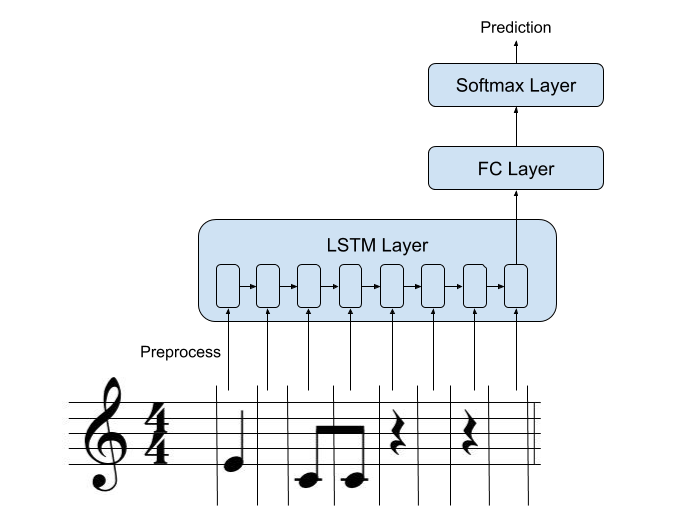
\includegraphics[width=0.5\textwidth]{Architecture.png}

The input sequence is then passed into an LSTM layer. We found that using a 150 length hidden state vector achieved the best results over our validation dataset. The final output of the LSTM layer is then passed into a fully connected linear layer, and finally into a softmax layer to compute the probabilities for each composer. We then pick the composer with the highest probability as the final result for the phrase. To increase accuracy over the whole musical piece, we take a majority vote over all the pharses in the piece. For the rest of this paper, we refer to ``phrase accuracy'' as accuracy for 1 phrase, while ``piece accuracy'' is the accuracy for each piece after taking this majority. 

To train the network, we use mini-batches of size 500 and the Adam optimizer with a decaying learning rate. Since our dataset is highly imbalanced (we have several times more examples from Beethoven/Bach than lesser known composers), we oversample the composers with fewer unique examples to compensate. The optimizer is set to minimize the cross entropy error over the training dataset. Our deep learning implementation was done in TensorFlow.


\section{Experiments and Results}

\subsection{Data}
In this paper we use the KernScores database which contains musical pieces as a MIDI files. The KernScores database is a large collection of virtual musical scores made available by the Center for Computer Assisted Research in the humanities at Stanford University (CCARH). The KernScores database has a total of $7,866,496$ notes and is available online at \texttt{kern.ccarh.org} 

As a baseline, we aim to compare our results with the 86\% accuracy result from Herremans, Sorensen, and Martens \cite {Herremans}. They also used the KernScores dataset and achieved fairly good accuracy. Their work attempts to solve multiclass classification between Bach, Beethoven, and Haydn, so we also chose these composers in our experimental results. An overview of the selected composers was given in table 1.

\begin{table}[t!]
\begin{center}
\begin{tabular}{|l|l|}
\hline \bf Composers & \bf Examples \\ \hline
Beethoven & 10526 \\
Haydn & 9758 \\
Bach & 8544\\
Corelli & 3555\\
Buxtehude & 3728\\
Monteverdi & 302 \\
Foster & 350\\
Frescobaldi & 1904\\
Josquin & 79\\
Schumann & 82\\
Joplin & 1788\\
Gershwin & 890\\
Giovannelli & 139\\
Mozart & 6733  \\
\hline
\end{tabular}
\end{center}
\caption{\label{composer-table}List of composers. }
\end{table}


\subsection{Experiments}
% Young: TODO
We ran this model on a "add the machine info" . The other information regarding our architecture are listed in table 2.

\begin{table}[t!]
\begin{center}
\begin{tabular}{|l|l|}
\hline \bf Specification & \bf Value\\ \hline
Batch size & 500 \\
Learning rate & 0.01\\
Hidden state & 150\\
\hline
\end{tabular}
\end{center}
\caption{\label{arch-specification-table}Architecture Specification. }
\end{table}
\subsection{Results}
Most previous work identifies a composer from an entire piece, so to properly evaluate our model we should compare our piece accuracy against the other models. Our results show that our model achieves an accuracy of 87.3\% on Beethoven, Bach, and Haydn, and 1.3\% improvement over the previous work. % Young: Add some comments about individual composers maybe? Or other comments

In addition to the 3 composer case, we also ran some experiments to see if our classifier generalizes to more composers from a wider range of styles. Using the 10 selected composers above, we were able to achieve an accuracy of 72\% using the same model. Table 3 presents the accuracy for each composer. Interestingly, the lowest accuracy over all composers is Mozart. We believe this is because his musical style was highly variable and the body of work is vast, which makes it difficult for our model to nail down his style quantitatively.

\begin{table}[t!]
\begin{center}
\begin{tabular}{|l|l|}
\hline \bf Method & \bf Accuracy (\%) \\ \hline
\underline{LSTM} & 87.3 \\
Support vector machines & 86 \\
Logistic regression & 83\\
C4.5 decision tree & 79\\
RIPPER rule set & 77\\
\hline
\end{tabular}
\end{center}
\caption{\label{resutls-table} Model Evaluation. }
\end{table}

% Young: Add phrase accuracy to the table below. Also include a similar one for the 3 composer case

\begin{table}[t!]
\begin{center}
\begin{tabular}{|l|l|}
\hline \bf Composers & \bf Accuracy (\%)\\ \hline
Beethoven & 72 \\
Mozart & 47\\
Foster & 59\\
Frescobaldi & 99\\
Josquin & 65\\
Schumann & 62\\
Joplin & 93\\
Gershwin & 95\\
Giovannelli & 96\\
Vivaldi & 95  \\
\hline
\end{tabular}
\end{center}
\caption{\label{test-accuracy-table}Accuracy. }
\end{table}

% X axis is unlabeled for these graphs. Is this the 10 composer or 3 composer case? Maybe add graphs for both?

\begin{figure}[h]
\caption{Piece Accuracy Training Curve}
\centering
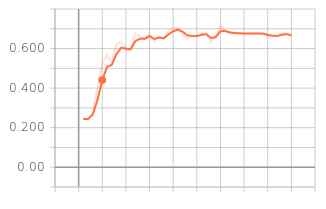
\includegraphics[width=0.5\textwidth]{Gaccuracy.png}
\end{figure}

\begin{figure}[h]
\caption{Phrase Accuracy Training Curve}
\centering
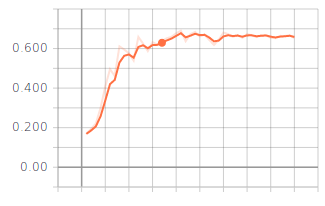
\includegraphics[width=0.5\textwidth]{vaccuracy.png}
\end{figure}


\section{Conclusion and Future Work}
% Young: TODO

The development of musical grammar shows that there is a hierarchical structures in a musical component. Over the years, researchers around the world tried to classify musical pieces based on these hierarchical structures. With the advances in computers and technologies, researchers started classifying pieces using computers. In this paper, we tackled the question "Can computers accurately identify the composer of a musical piece?". The result is an LSTM model that is capable of identifying the composer of each musical piece. We were able to build a model that surpass the previous state of the art approach by 1.3\%. Our approach is generalized to work on a larger list of composers compared to previous approaches. 

As for future work, we would like to have an explicit feature extraction. We believe having the right features has a high impact on the accuracy of our model. We would also like to study each composers in depth and have a collaboration with a few music theorist to build a better model. Also, currentely we have a multi-class classifier. We would like to expand our work and build a binary classifier as well were we can tell if a musical piece is a work of specific composer. 



\bibliography{emnlp2018}
\bibliographystyle{acl_natbib_nourl}

\appendix



Appendices ({\em i.e.} supplementary material in the form of proofs, tables,
or pseudo-code) should be {\bf uploaded as supplementary material} when submitting the paper for review.
Upon acceptance, the appendices come after the references, as shown here. Use
\verb|\appendix| before any appendix section to switch the section
numbering over to letters.

\end{document}
